\documentclass[1p]{elsarticle_modified}
%\bibliographystyle{elsarticle-num}

%\usepackage[colorlinks]{hyperref}
%\usepackage{abbrmath_seonhwa} %\Abb, \Ascr, \Acal ,\Abf, \Afrak
\usepackage{amsfonts}
\usepackage{amssymb}
\usepackage{amsmath}
\usepackage{amsthm}
\usepackage{scalefnt}
\usepackage{amsbsy}
\usepackage{kotex}
\usepackage{caption}
\usepackage{subfig}
\usepackage{color}
\usepackage{graphicx}
\usepackage{xcolor} %% white, black, red, green, blue, cyan, magenta, yellow
\usepackage{float}
\usepackage{setspace}
\usepackage{hyperref}

\usepackage{tikz}
\usetikzlibrary{arrows}

\usepackage{multirow}
\usepackage{array} % fixed length table
\usepackage{hhline}

%%%%%%%%%%%%%%%%%%%%%
\makeatletter
\renewcommand*\env@matrix[1][\arraystretch]{%
	\edef\arraystretch{#1}%
	\hskip -\arraycolsep
	\let\@ifnextchar\new@ifnextchar
	\array{*\c@MaxMatrixCols c}}
\makeatother %https://tex.stackexchange.com/questions/14071/how-can-i-increase-the-line-spacing-in-a-matrix
%%%%%%%%%%%%%%%

\usepackage[normalem]{ulem}

\newcommand{\msout}[1]{\ifmmode\text{\sout{\ensuremath{#1}}}\else\sout{#1}\fi}
%SOURCE: \msout is \stkout macro in https://tex.stackexchange.com/questions/20609/strikeout-in-math-mode

\newcommand{\cancel}[1]{
	\ifmmode
	{\color{red}\msout{#1}}
	\else
	{\color{red}\sout{#1}}
	\fi
}

\newcommand{\add}[1]{
	{\color{blue}\uwave{#1}}
}

\newcommand{\replace}[2]{
	\ifmmode
	{\color{red}\msout{#1}}{\color{blue}\uwave{#2}}
	\else
	{\color{red}\sout{#1}}{\color{blue}\uwave{#2}}
	\fi
}

\newcommand{\Sol}{\mathcal{S}} %segment
\newcommand{\D}{D} %diagram
\newcommand{\A}{\mathcal{A}} %arc


%%%%%%%%%%%%%%%%%%%%%%%%%%%%%5 test

\def\sl{\operatorname{\textup{SL}}(2,\Cbb)}
\def\psl{\operatorname{\textup{PSL}}(2,\Cbb)}
\def\quan{\mkern 1mu \triangleright \mkern 1mu}

\theoremstyle{definition}
\newtheorem{thm}{Theorem}[section]
\newtheorem{prop}[thm]{Proposition}
\newtheorem{lem}[thm]{Lemma}
\newtheorem{ques}[thm]{Question}
\newtheorem{cor}[thm]{Corollary}
\newtheorem{defn}[thm]{Definition}
\newtheorem{exam}[thm]{Example}
\newtheorem{rmk}[thm]{Remark}
\newtheorem{alg}[thm]{Algorithm}

\newcommand{\I}{\sqrt{-1}}
\begin{document}

%\begin{frontmatter}
%
%\title{Boundary parabolic representations of knots up to 8 crossings}
%
%%% Group authors per affiliation:
%\author{Yunhi Cho} 
%\address{Department of Mathematics, University of Seoul, Seoul, Korea}
%\ead{yhcho@uos.ac.kr}
%
%
%\author{Seonhwa Kim} %\fnref{s_kim}}
%\address{Center for Geometry and Physics, Institute for Basic Science, Pohang, 37673, Korea}
%\ead{ryeona17@ibs.re.kr}
%
%\author{Hyuk Kim}
%\address{Department of Mathematical Sciences, Seoul National University, Seoul 08826, Korea}
%\ead{hyukkim@snu.ac.kr}
%
%\author{Seokbeom Yoon}
%\address{Department of Mathematical Sciences, Seoul National University, Seoul, 08826,  Korea}
%\ead{sbyoon15@snu.ac.kr}
%
%\begin{abstract}
%We find all boundary parabolic representation of knots up to 8 crossings.
%
%\end{abstract}
%\begin{keyword}
%    \MSC[2010] 57M25 
%\end{keyword}
%
%\end{frontmatter}

%\linenumbers
%\tableofcontents
%
\newcommand\colored[1]{\textcolor{white}{\rule[-0.35ex]{0.8em}{1.4ex}}\kern-0.8em\color{red} #1}%
%\newcommand\colored[1]{\textcolor{white}{ #1}\kern-2.17ex	\textcolor{white}{ #1}\kern-1.81ex	\textcolor{white}{ #1}\kern-2.15ex\color{red}#1	}

{\Large $\underline{12n_{0845}~(K12n_{0845})}$}

\setlength{\tabcolsep}{10pt}
\renewcommand{\arraystretch}{1.6}
\vspace{1cm}\begin{tabular}{m{100pt}>{\centering\arraybackslash}m{274pt}}
\multirow{5}{120pt}{
	\centering
	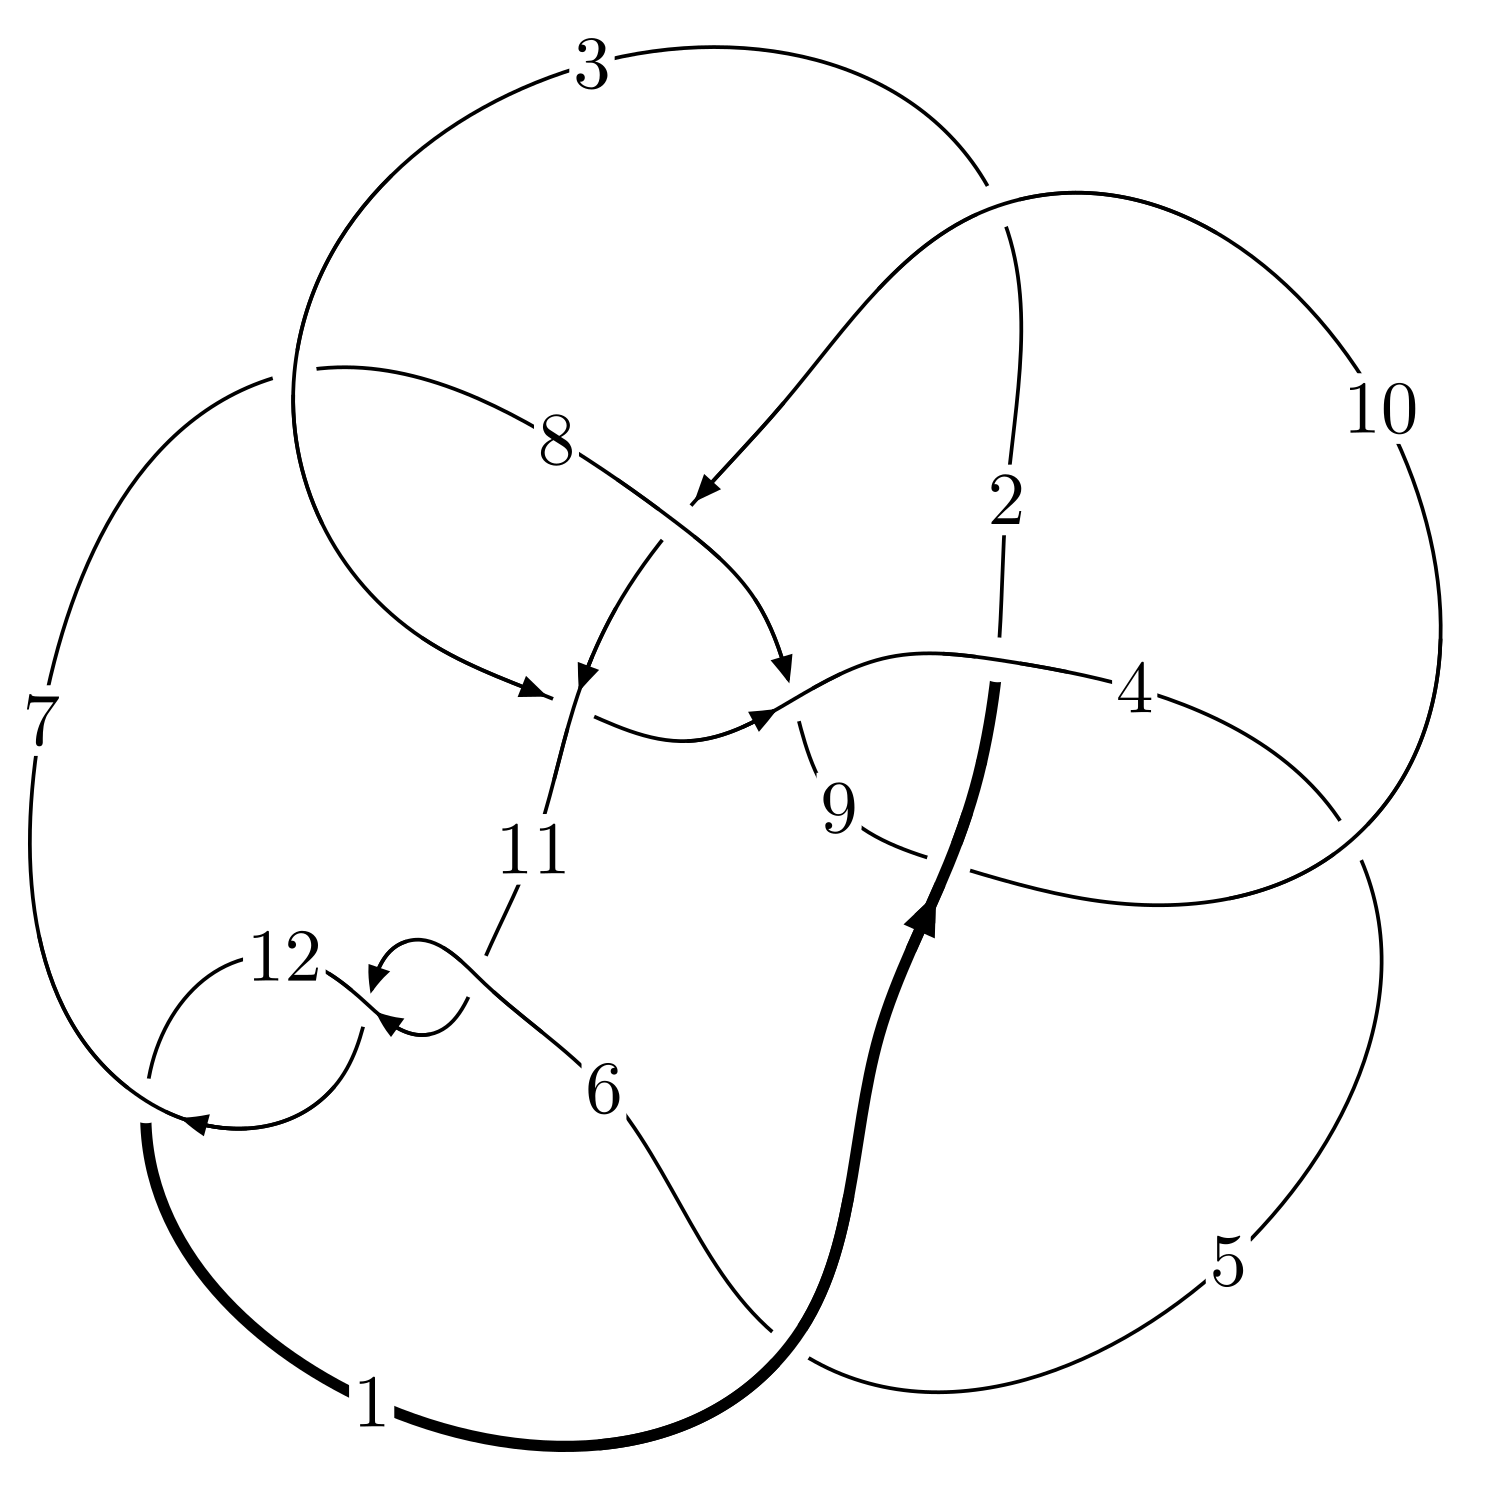
\includegraphics[width=112pt]{../../../GIT/diagram.site/Diagrams/png/2934_12n_0845.png}\\
\ \ \ A knot diagram\footnotemark}&
\allowdisplaybreaks
\textbf{Linearized knot diagam} \\
\cline{2-2}
 &
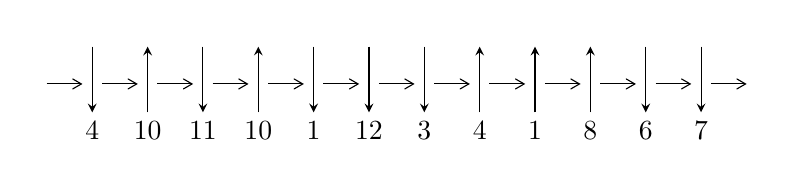
\begin{tikzpicture}[x=20pt, y=17pt]
	% nodes
	\node (C0) at (0, 0) {};
	\node (C1) at (1, 0) {};
	\node (C1U) at (1, +1) {};
	\node (C1D) at (1, -1) {4};

	\node (C2) at (2, 0) {};
	\node (C2U) at (2, +1) {};
	\node (C2D) at (2, -1) {10};

	\node (C3) at (3, 0) {};
	\node (C3U) at (3, +1) {};
	\node (C3D) at (3, -1) {11};

	\node (C4) at (4, 0) {};
	\node (C4U) at (4, +1) {};
	\node (C4D) at (4, -1) {10};

	\node (C5) at (5, 0) {};
	\node (C5U) at (5, +1) {};
	\node (C5D) at (5, -1) {1};

	\node (C6) at (6, 0) {};
	\node (C6U) at (6, +1) {};
	\node (C6D) at (6, -1) {12};

	\node (C7) at (7, 0) {};
	\node (C7U) at (7, +1) {};
	\node (C7D) at (7, -1) {3};

	\node (C8) at (8, 0) {};
	\node (C8U) at (8, +1) {};
	\node (C8D) at (8, -1) {4};

	\node (C9) at (9, 0) {};
	\node (C9U) at (9, +1) {};
	\node (C9D) at (9, -1) {1};

	\node (C10) at (10, 0) {};
	\node (C10U) at (10, +1) {};
	\node (C10D) at (10, -1) {8};

	\node (C11) at (11, 0) {};
	\node (C11U) at (11, +1) {};
	\node (C11D) at (11, -1) {6};

	\node (C12) at (12, 0) {};
	\node (C12U) at (12, +1) {};
	\node (C12D) at (12, -1) {7};
	\node (C13) at (13, 0) {};

	% arrows
	\draw[->,>={angle 60}]
	(C0) edge (C1) (C1) edge (C2) (C2) edge (C3) (C3) edge (C4) (C4) edge (C5) (C5) edge (C6) (C6) edge (C7) (C7) edge (C8) (C8) edge (C9) (C9) edge (C10) (C10) edge (C11) (C11) edge (C12) (C12) edge (C13) ;	\draw[->,>=stealth]
	(C1U) edge (C1D) (C2D) edge (C2U) (C3U) edge (C3D) (C4D) edge (C4U) (C5U) edge (C5D) (C6U) edge (C6D) (C7U) edge (C7D) (C8D) edge (C8U) (C9D) edge (C9U) (C10D) edge (C10U) (C11U) edge (C11D) (C12U) edge (C12D) ;
	\end{tikzpicture} \\
\hhline{~~} \\& 
\textbf{Solving Sequence} \\ \cline{2-2} 
 &
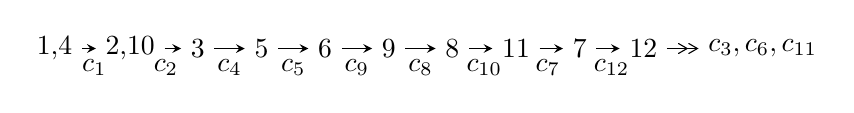
\begin{tikzpicture}[x=23pt, y=7pt]
	% node
	\node (A0) at (-1/8, 0) {1,4};
	\node (A1) at (17/16, 0) {2,10};
	\node (A2) at (17/8, 0) {3};
	\node (A3) at (25/8, 0) {5};
	\node (A4) at (33/8, 0) {6};
	\node (A5) at (41/8, 0) {9};
	\node (A6) at (49/8, 0) {8};
	\node (A7) at (57/8, 0) {11};
	\node (A8) at (65/8, 0) {7};
	\node (A9) at (73/8, 0) {12};
	\node (C1) at (1/2, -1) {$c_{1}$};
	\node (C2) at (13/8, -1) {$c_{2}$};
	\node (C3) at (21/8, -1) {$c_{4}$};
	\node (C4) at (29/8, -1) {$c_{5}$};
	\node (C5) at (37/8, -1) {$c_{9}$};
	\node (C6) at (45/8, -1) {$c_{8}$};
	\node (C7) at (53/8, -1) {$c_{10}$};
	\node (C8) at (61/8, -1) {$c_{7}$};
	\node (C9) at (69/8, -1) {$c_{12}$};
	\node (A10) at (11, 0) {$c_{3},c_{6},c_{11}$};

	% edge
	\draw[->,>=stealth]	
	(A0) edge (A1) (A1) edge (A2) (A2) edge (A3) (A3) edge (A4) (A4) edge (A5) (A5) edge (A6) (A6) edge (A7) (A7) edge (A8) (A8) edge (A9) ;
	\draw[->>,>={angle 60}]	
	(A9) edge (A10);
\end{tikzpicture} \\ 

\end{tabular} \\

\footnotetext{
The image of knot diagram is generated by the software ``\textbf{Draw programme}" developed by Andrew Bartholomew(\url{http://www.layer8.co.uk/maths/draw/index.htm\#Running-draw}), where we modified some parts for our purpose(\url{https://github.com/CATsTAILs/LinksPainter}).
}\phantom \\ \newline 
\centering \textbf{Ideals for irreducible components\footnotemark of $X_{\text{par}}$} 
 
\begin{align*}
I^u_{1}&=\langle 
7.47941\times10^{24} u^{27}+1.23843\times10^{26} u^{26}+\cdots+1.61992\times10^{22} b+5.31574\times10^{27},\\
\phantom{I^u_{1}}&\phantom{= \langle  }1.03823\times10^{25} u^{27}+1.71923\times10^{26} u^{26}+\cdots+3.23983\times10^{22} a+7.38572\times10^{27},\\
\phantom{I^u_{1}}&\phantom{= \langle  }u^{28}+18 u^{27}+\cdots+1280 u+1024\rangle \\
I^u_{2}&=\langle 
-7125076710 u^{18}+91561872113 u^{17}+\cdots+543606477 b-93548383993,\\
\phantom{I^u_{2}}&\phantom{= \langle  }-93548383993 u^{18}+1209003915199 u^{17}+\cdots+543606477 a-1268729042138,\\
\phantom{I^u_{2}}&\phantom{= \langle  }u^{19}-13 u^{18}+\cdots+29 u-1\rangle \\
I^u_{3}&=\langle 
468422399 a^9 u^3+40467670 a^8 u^3+\cdots-48741327 a+38855139,\\
\phantom{I^u_{3}}&\phantom{= \langle  }- a^9 u^3-9 a^8 u^3+\cdots+679 a-378,\;u^4-3 u^3+u^2+2 u+1\rangle \\
\\
\end{align*}
\raggedright * 3 irreducible components of $\dim_{\mathbb{C}}=0$, with total 87 representations.\\
\footnotetext{All coefficients of polynomials are rational numbers. But the coefficients are sometimes approximated in decimal forms when there is not enough margin.}
\newpage
\renewcommand{\arraystretch}{1}
\centering \section*{I. $I^u_{1}= \langle 7.48\times10^{24} u^{27}+1.24\times10^{26} u^{26}+\cdots+1.62\times10^{22} b+5.32\times10^{27},\;1.04\times10^{25} u^{27}+1.72\times10^{26} u^{26}+\cdots+3.24\times10^{22} a+7.39\times10^{27},\;u^{28}+18 u^{27}+\cdots+1280 u+1024 \rangle$}
\flushleft \textbf{(i) Arc colorings}\\
\begin{tabular}{m{7pt} m{180pt} m{7pt} m{180pt} }
\flushright $a_{1}=$&$\begin{pmatrix}1\\0\end{pmatrix}$ \\
\flushright $a_{4}=$&$\begin{pmatrix}0\\u\end{pmatrix}$ \\
\flushright $a_{2}=$&$\begin{pmatrix}1\\u^2\end{pmatrix}$ \\
\flushright $a_{10}=$&$\begin{pmatrix}-320.458 u^{27}-5306.53 u^{26}+\cdots-126445. u-227966.\\-461.716 u^{27}-7645.01 u^{26}+\cdots-182220. u-328149.\end{pmatrix}$ \\
\flushright $a_{3}=$&$\begin{pmatrix}-37.8334 u^{27}-632.042 u^{26}+\cdots-14648.4 u-29529.5\\-48.9592 u^{27}-819.012 u^{26}+\cdots-18896.2 u-38741.4\end{pmatrix}$ \\
\flushright $a_{5}=$&$\begin{pmatrix}111.460 u^{27}+1856.99 u^{26}+\cdots+43415.8 u+84604.4\\149.293 u^{27}+2489.03 u^{26}+\cdots+58065.3 u+114135.\end{pmatrix}$ \\
\flushright $a_{6}=$&$\begin{pmatrix}-37.8334 u^{27}-632.042 u^{26}+\cdots-14649.4 u-29530.5\\149.293 u^{27}+2489.03 u^{26}+\cdots+58065.3 u+114135.\end{pmatrix}$ \\
\flushright $a_{9}=$&$\begin{pmatrix}141.258 u^{27}+2338.48 u^{26}+\cdots+55775.1 u+100183.\\-461.716 u^{27}-7645.01 u^{26}+\cdots-182220. u-328149.\end{pmatrix}$ \\
\flushright $a_{8}=$&$\begin{pmatrix}141.258 u^{27}+2338.48 u^{26}+\cdots+55775.1 u+100183.\\-166.322 u^{27}-2755.77 u^{26}+\cdots-65538.3 u-119085.\end{pmatrix}$ \\
\flushright $a_{11}=$&$\begin{pmatrix}-81.7198 u^{27}-1353.54 u^{26}+\cdots-32166.5 u-58365.7\\-746.494 u^{27}-12362.3 u^{26}+\cdots-294547. u-531430.\end{pmatrix}$ \\
\flushright $a_{7}=$&$\begin{pmatrix}205.704 u^{27}+3402.49 u^{26}+\cdots+81390.4 u+144506.\\-145.362 u^{27}-2412.32 u^{26}+\cdots-56976.3 u-106020.\end{pmatrix}$ \\
\flushright $a_{12}=$&$\begin{pmatrix}-103.259 u^{27}-1702.27 u^{26}+\cdots-41159.1 u-69833.4\\-208.655 u^{27}-3462.18 u^{26}+\cdots-82098.9 u-151590.\end{pmatrix}$\\&\end{tabular}
\flushleft \textbf{(ii) Obstruction class $= -1$}\\~\\
\flushleft \textbf{(iii) Cusp Shapes $= \frac{13322328677737983134489147}{8099581639968855113536} u^{27}+\frac{110674001941628848158963191}{4049790819984427556768} u^{26}+\cdots+\frac{81474007049283441507399205}{126555963124513361149} u+\frac{153623166708123437656283814}{126555963124513361149}$}\\~\\
\newpage\renewcommand{\arraystretch}{1}
\flushleft \textbf{(iv) u-Polynomials at the component}\newline \\
\begin{tabular}{m{50pt}|m{274pt}}
Crossings & \hspace{64pt}u-Polynomials at each crossing \\
\hline $$\begin{aligned}c_{1}\end{aligned}$$&$\begin{aligned}
&u^{28}-18 u^{27}+\cdots-1280 u+1024
\end{aligned}$\\
\hline $$\begin{aligned}c_{2},c_{8}\end{aligned}$$&$\begin{aligned}
&u^{28}+u^{27}+\cdots+2 u+10
\end{aligned}$\\
\hline $$\begin{aligned}c_{3},c_{7}\end{aligned}$$&$\begin{aligned}
&u^{28}-3 u^{26}+\cdots-4 u+1
\end{aligned}$\\
\hline $$\begin{aligned}c_{4},c_{9}\end{aligned}$$&$\begin{aligned}
&u^{28}+u^{27}+\cdots+2 u+1
\end{aligned}$\\
\hline $$\begin{aligned}c_{5}\end{aligned}$$&$\begin{aligned}
&u^{28}+27 u^{27}+\cdots+186016 u+13840
\end{aligned}$\\
\hline $$\begin{aligned}c_{6},c_{11},c_{12}\end{aligned}$$&$\begin{aligned}
&u^{28}-8 u^{27}+\cdots+32 u+16
\end{aligned}$\\
\hline $$\begin{aligned}c_{10}\end{aligned}$$&$\begin{aligned}
&u^{28}+21 u^{27}+\cdots+432 u+32
\end{aligned}$\\
\hline
\end{tabular}\\~\\
\newpage\renewcommand{\arraystretch}{1}
\flushleft \textbf{(v) Riley Polynomials at the component}\newline \\
\begin{tabular}{m{50pt}|m{274pt}}
Crossings & \hspace{64pt}Riley Polynomials at each crossing \\
\hline $$\begin{aligned}c_{1}\end{aligned}$$&$\begin{aligned}
&y^{28}-28 y^{27}+\cdots+2162688 y+1048576
\end{aligned}$\\
\hline $$\begin{aligned}c_{2},c_{8}\end{aligned}$$&$\begin{aligned}
&y^{28}+17 y^{27}+\cdots+1336 y+100
\end{aligned}$\\
\hline $$\begin{aligned}c_{3},c_{7}\end{aligned}$$&$\begin{aligned}
&y^{28}-6 y^{27}+\cdots-22 y+1
\end{aligned}$\\
\hline $$\begin{aligned}c_{4},c_{9}\end{aligned}$$&$\begin{aligned}
&y^{28}+45 y^{27}+\cdots+16 y+1
\end{aligned}$\\
\hline $$\begin{aligned}c_{5}\end{aligned}$$&$\begin{aligned}
&y^{28}+3 y^{27}+\cdots-987913856 y+191545600
\end{aligned}$\\
\hline $$\begin{aligned}c_{6},c_{11},c_{12}\end{aligned}$$&$\begin{aligned}
&y^{28}-24 y^{27}+\cdots-640 y+256
\end{aligned}$\\
\hline $$\begin{aligned}c_{10}\end{aligned}$$&$\begin{aligned}
&y^{28}+5 y^{27}+\cdots+13568 y+1024
\end{aligned}$\\
\hline
\end{tabular}\\~\\
\newpage\flushleft \textbf{(vi) Complex Volumes and Cusp Shapes}
$$\begin{array}{c|c|c}  
\text{Solutions to }I^u_{1}& \I (\text{vol} + \sqrt{-1}CS) & \text{Cusp shape}\\
 \hline 
\begin{aligned}
u &= \phantom{-}0.425697 + 0.914932 I \\
a &= -0.312755 - 0.479893 I \\
b &= -0.305930 + 0.490439 I\end{aligned}
 & -3.34248 - 5.03502 I & \phantom{-0.000000 -}0. + 7.22973 I \\ \hline\begin{aligned}
u &= \phantom{-}0.425697 - 0.914932 I \\
a &= -0.312755 + 0.479893 I \\
b &= -0.305930 - 0.490439 I\end{aligned}
 & -3.34248 + 5.03502 I & \phantom{-0.000000 } 0. - 7.22973 I \\ \hline\begin{aligned}
u &= -0.105022 + 1.112840 I \\
a &= \phantom{-}0.381320 - 0.351416 I \\
b &= -0.351024 - 0.461256 I\end{aligned}
 & -0.514267 + 0.130456 I & \phantom{-0.000000 } 0 \\ \hline\begin{aligned}
u &= -0.105022 - 1.112840 I \\
a &= \phantom{-}0.381320 + 0.351416 I \\
b &= -0.351024 + 0.461256 I\end{aligned}
 & -0.514267 - 0.130456 I & \phantom{-0.000000 } 0 \\ \hline\begin{aligned}
u &= \phantom{-}1.130170 + 0.322911 I \\
a &= -0.317402 - 0.254746 I \\
b &= \phantom{-}0.276457 + 0.390398 I\end{aligned}
 & -6.73975 - 1.18993 I & \phantom{-0.000000 } 0 \\ \hline\begin{aligned}
u &= \phantom{-}1.130170 - 0.322911 I \\
a &= -0.317402 + 0.254746 I \\
b &= \phantom{-}0.276457 - 0.390398 I\end{aligned}
 & -6.73975 + 1.18993 I & \phantom{-0.000000 } 0 \\ \hline\begin{aligned}
u &= -1.324700 + 0.306113 I \\
a &= -0.621209 + 1.202590 I \\
b &= -0.45479 + 1.78323 I\end{aligned}
 & -5.26230 + 3.26030 I & \phantom{-0.000000 } 0 \\ \hline\begin{aligned}
u &= -1.324700 - 0.306113 I \\
a &= -0.621209 - 1.202590 I \\
b &= -0.45479 - 1.78323 I\end{aligned}
 & -5.26230 - 3.26030 I & \phantom{-0.000000 } 0 \\ \hline\begin{aligned}
u &= -1.41642 + 0.00861 I \\
a &= \phantom{-}0.253081 - 1.240320 I \\
b &= \phantom{-}0.34779 - 1.75900 I\end{aligned}
 & -3.54950 - 3.27899 I & \phantom{-0.000000 } 0 \\ \hline\begin{aligned}
u &= -1.41642 - 0.00861 I \\
a &= \phantom{-}0.253081 + 1.240320 I \\
b &= \phantom{-}0.34779 + 1.75900 I\end{aligned}
 & -3.54950 + 3.27899 I & \phantom{-0.000000 } 0\\
 \hline 
 \end{array}$$\newpage$$\begin{array}{c|c|c}  
\text{Solutions to }I^u_{1}& \I (\text{vol} + \sqrt{-1}CS) & \text{Cusp shape}\\
 \hline 
\begin{aligned}
u &= \phantom{-}0.040270 + 0.540835 I \\
a &= \phantom{-}0.764936 + 0.846392 I \\
b &= \phantom{-}0.426954 - 0.447789 I\end{aligned}
 & \phantom{-}0.86405 - 1.47972 I & \phantom{-}0.04127 + 5.19835 I \\ \hline\begin{aligned}
u &= \phantom{-}0.040270 - 0.540835 I \\
a &= \phantom{-}0.764936 - 0.846392 I \\
b &= \phantom{-}0.426954 + 0.447789 I\end{aligned}
 & \phantom{-}0.86405 + 1.47972 I & \phantom{-}0.04127 - 5.19835 I \\ \hline\begin{aligned}
u &= \phantom{-}0.31182 + 1.46661 I \\
a &= -0.308577 + 0.173644 I \\
b &= \phantom{-}0.350888 + 0.398418 I\end{aligned}
 & \phantom{-}2.48566 - 3.77616 I & \phantom{-0.000000 } 0 \\ \hline\begin{aligned}
u &= \phantom{-}0.31182 - 1.46661 I \\
a &= -0.308577 - 0.173644 I \\
b &= \phantom{-}0.350888 - 0.398418 I\end{aligned}
 & \phantom{-}2.48566 + 3.77616 I & \phantom{-0.000000 } 0 \\ \hline\begin{aligned}
u &= -1.52883 + 0.03670 I \\
a &= -0.339231 - 1.169130 I \\
b &= -0.56153 - 1.77495 I\end{aligned}
 & -9.73727 + 7.90821 I & \phantom{-0.000000 } 0 \\ \hline\begin{aligned}
u &= -1.52883 - 0.03670 I \\
a &= -0.339231 + 1.169130 I \\
b &= -0.56153 + 1.77495 I\end{aligned}
 & -9.73727 - 7.90821 I & \phantom{-0.000000 } 0 \\ \hline\begin{aligned}
u &= \phantom{-}0.332678 + 0.259381 I \\
a &= \phantom{-}1.059500 + 0.353725 I \\
b &= -0.260723 - 0.392490 I\end{aligned}
 & -1.017830 - 0.678910 I & -6.84852 + 2.35129 I \\ \hline\begin{aligned}
u &= \phantom{-}0.332678 - 0.259381 I \\
a &= \phantom{-}1.059500 - 0.353725 I \\
b &= -0.260723 + 0.392490 I\end{aligned}
 & -1.017830 + 0.678910 I & -6.84852 - 2.35129 I \\ \hline\begin{aligned}
u &= -1.73874 + 0.31279 I \\
a &= \phantom{-}0.195104 - 1.130570 I \\
b &= -0.01440 - 2.02680 I\end{aligned}
 & -15.5874 + 4.5388 I & \phantom{-0.000000 } 0 \\ \hline\begin{aligned}
u &= -1.73874 - 0.31279 I \\
a &= \phantom{-}0.195104 + 1.130570 I \\
b &= -0.01440 + 2.02680 I\end{aligned}
 & -15.5874 - 4.5388 I & \phantom{-0.000000 } 0\\
 \hline 
 \end{array}$$\newpage$$\begin{array}{c|c|c}  
\text{Solutions to }I^u_{1}& \I (\text{vol} + \sqrt{-1}CS) & \text{Cusp shape}\\
 \hline 
\begin{aligned}
u &= \phantom{-}0.62542 + 1.66377 I \\
a &= \phantom{-}0.263163 - 0.106601 I \\
b &= -0.341946 - 0.371174 I\end{aligned}
 & -2.13746 - 7.74211 I & \phantom{-0.000000 } 0 \\ \hline\begin{aligned}
u &= \phantom{-}0.62542 - 1.66377 I \\
a &= \phantom{-}0.263163 + 0.106601 I \\
b &= -0.341946 + 0.371174 I\end{aligned}
 & -2.13746 + 7.74211 I & \phantom{-0.000000 } 0 \\ \hline\begin{aligned}
u &= -1.83553 + 0.47211 I \\
a &= -0.097425 + 0.937524 I \\
b &= \phantom{-}0.26379 + 1.76685 I\end{aligned}
 & -7.04260 + 6.51785 I & \phantom{-0.000000 } 0 \\ \hline\begin{aligned}
u &= -1.83553 - 0.47211 I \\
a &= -0.097425 - 0.937524 I \\
b &= \phantom{-}0.26379 - 1.76685 I\end{aligned}
 & -7.04260 - 6.51785 I & \phantom{-0.000000 } 0 \\ \hline\begin{aligned}
u &= -1.93764 + 0.44814 I \\
a &= -0.023604 - 0.925470 I \\
b &= -0.46048 - 1.78265 I\end{aligned}
 & -5.47616 + 11.59450 I & \phantom{-0.000000 } 0 \\ \hline\begin{aligned}
u &= -1.93764 - 0.44814 I \\
a &= -0.023604 + 0.925470 I \\
b &= -0.46048 + 1.78265 I\end{aligned}
 & -5.47616 - 11.59450 I & \phantom{-0.000000 } 0 \\ \hline\begin{aligned}
u &= -1.97916 + 0.39645 I \\
a &= \phantom{-}0.103098 + 0.960765 I \\
b &= \phantom{-}0.58495 + 1.86064 I\end{aligned}
 & -11.2075 + 15.9109 I & \phantom{-0.000000 } 0 \\ \hline\begin{aligned}
u &= -1.97916 - 0.39645 I \\
a &= \phantom{-}0.103098 - 0.960765 I \\
b &= \phantom{-}0.58495 - 1.86064 I\end{aligned}
 & -11.2075 - 15.9109 I & \phantom{-0.000000 } 0\\
 \hline 
 \end{array}$$\newpage\newpage\renewcommand{\arraystretch}{1}
\centering \section*{II. $I^u_{2}= \langle -7.13\times10^{9} u^{18}+9.16\times10^{10} u^{17}+\cdots+5.44\times10^{8} b-9.35\times10^{10},\;-9.35\times10^{10} u^{18}+1.21\times10^{12} u^{17}+\cdots+5.44\times10^{8} a-1.27\times10^{12},\;u^{19}-13 u^{18}+\cdots+29 u-1 \rangle$}
\flushleft \textbf{(i) Arc colorings}\\
\begin{tabular}{m{7pt} m{180pt} m{7pt} m{180pt} }
\flushright $a_{1}=$&$\begin{pmatrix}1\\0\end{pmatrix}$ \\
\flushright $a_{4}=$&$\begin{pmatrix}0\\u\end{pmatrix}$ \\
\flushright $a_{2}=$&$\begin{pmatrix}1\\u^2\end{pmatrix}$ \\
\flushright $a_{10}=$&$\begin{pmatrix}172.088 u^{18}-2224.04 u^{17}+\cdots-36002.5 u+2333.91\\13.1070 u^{18}-168.434 u^{17}+\cdots-2656.65 u+172.088\end{pmatrix}$ \\
\flushright $a_{3}=$&$\begin{pmatrix}-255.016 u^{18}+3296.25 u^{17}+\cdots+53367.8 u-3449.13\\-18.9607 u^{18}+244.839 u^{17}+\cdots+3945.33 u-255.016\end{pmatrix}$ \\
\flushright $a_{5}=$&$\begin{pmatrix}275.389 u^{18}-3559.68 u^{17}+\cdots-57628.5 u+3725.52\\20.3725 u^{18}-263.431 u^{17}+\cdots-4259.75 u+275.389\end{pmatrix}$ \\
\flushright $a_{6}=$&$\begin{pmatrix}255.016 u^{18}-3296.25 u^{17}+\cdots-53368.8 u+3450.13\\20.3725 u^{18}-263.431 u^{17}+\cdots-4259.75 u+275.389\end{pmatrix}$ \\
\flushright $a_{9}=$&$\begin{pmatrix}158.981 u^{18}-2055.61 u^{17}+\cdots-33345.8 u+2161.82\\13.1070 u^{18}-168.434 u^{17}+\cdots-2656.65 u+172.088\end{pmatrix}$ \\
\flushright $a_{8}=$&$\begin{pmatrix}158.981 u^{18}-2055.61 u^{17}+\cdots-33345.8 u+2161.82\\12.7663 u^{18}-166.395 u^{17}+\cdots-2821.01 u+183.238\end{pmatrix}$ \\
\flushright $a_{11}=$&$\begin{pmatrix}-386.578 u^{18}+4997.30 u^{17}+\cdots+80922.8 u-5216.60\\-34.7026 u^{18}+449.189 u^{17}+\cdots+7326.27 u-472.582\end{pmatrix}$ \\
\flushright $a_{7}=$&$\begin{pmatrix}239.348 u^{18}-3094.91 u^{17}+\cdots-50207.9 u+3243.13\\21.1566 u^{18}-274.000 u^{17}+\cdots-4496.28 u+290.649\end{pmatrix}$ \\
\flushright $a_{12}=$&$\begin{pmatrix}-155.007 u^{18}+2004.69 u^{17}+\cdots+32544.1 u-2096.72\\-14.7054 u^{18}+190.365 u^{17}+\cdots+3100.48 u-199.857\end{pmatrix}$\\&\end{tabular}
\flushleft \textbf{(ii) Obstruction class $= 1$}\\~\\
\flushleft \textbf{(iii) Cusp Shapes $= -\frac{119077780094}{543606477} u^{18}+\frac{513494948917}{181202159} u^{17}+\cdots+\frac{25027294000157}{543606477} u-\frac{1610829968363}{543606477}$}\\~\\
\newpage\renewcommand{\arraystretch}{1}
\flushleft \textbf{(iv) u-Polynomials at the component}\newline \\
\begin{tabular}{m{50pt}|m{274pt}}
Crossings & \hspace{64pt}u-Polynomials at each crossing \\
\hline $$\begin{aligned}c_{1}\end{aligned}$$&$\begin{aligned}
&u^{19}-13 u^{18}+\cdots+29 u-1
\end{aligned}$\\
\hline $$\begin{aligned}c_{2},c_{8}\end{aligned}$$&$\begin{aligned}
&u^{19}- u^{18}+\cdots+15 u+4
\end{aligned}$\\
\hline $$\begin{aligned}c_{3},c_{7}\end{aligned}$$&$\begin{aligned}
&u^{19}+3 u^{17}+\cdots-5 u-1
\end{aligned}$\\
\hline $$\begin{aligned}c_{4},c_{9}\end{aligned}$$&$\begin{aligned}
&u^{19}- u^{18}+\cdots- u-1
\end{aligned}$\\
\hline $$\begin{aligned}c_{5}\end{aligned}$$&$\begin{aligned}
&u^{19}+2 u^{17}+\cdots- u+2
\end{aligned}$\\
\hline $$\begin{aligned}c_{6}\end{aligned}$$&$\begin{aligned}
&u^{19}- u^{18}+\cdots+u-2
\end{aligned}$\\
\hline $$\begin{aligned}c_{10}\end{aligned}$$&$\begin{aligned}
&u^{19}-6 u^{18}+\cdots- u^2-1
\end{aligned}$\\
\hline $$\begin{aligned}c_{11},c_{12}\end{aligned}$$&$\begin{aligned}
&u^{19}+u^{18}+\cdots+u+2
\end{aligned}$\\
\hline
\end{tabular}\\~\\
\newpage\renewcommand{\arraystretch}{1}
\flushleft \textbf{(v) Riley Polynomials at the component}\newline \\
\begin{tabular}{m{50pt}|m{274pt}}
Crossings & \hspace{64pt}Riley Polynomials at each crossing \\
\hline $$\begin{aligned}c_{1}\end{aligned}$$&$\begin{aligned}
&y^{19}-21 y^{18}+\cdots+369 y-1
\end{aligned}$\\
\hline $$\begin{aligned}c_{2},c_{8}\end{aligned}$$&$\begin{aligned}
&y^{19}+9 y^{18}+\cdots+313 y-16
\end{aligned}$\\
\hline $$\begin{aligned}c_{3},c_{7}\end{aligned}$$&$\begin{aligned}
&y^{19}+6 y^{18}+\cdots+13 y-1
\end{aligned}$\\
\hline $$\begin{aligned}c_{4},c_{9}\end{aligned}$$&$\begin{aligned}
&y^{19}+13 y^{18}+\cdots+15 y-1
\end{aligned}$\\
\hline $$\begin{aligned}c_{5}\end{aligned}$$&$\begin{aligned}
&y^{19}+4 y^{18}+\cdots-7 y-4
\end{aligned}$\\
\hline $$\begin{aligned}c_{6},c_{11},c_{12}\end{aligned}$$&$\begin{aligned}
&y^{19}-19 y^{18}+\cdots-7 y-4
\end{aligned}$\\
\hline $$\begin{aligned}c_{10}\end{aligned}$$&$\begin{aligned}
&y^{19}+4 y^{18}+\cdots-2 y-1
\end{aligned}$\\
\hline
\end{tabular}\\~\\
\newpage\flushleft \textbf{(vi) Complex Volumes and Cusp Shapes}
$$\begin{array}{c|c|c}  
\text{Solutions to }I^u_{2}& \I (\text{vol} + \sqrt{-1}CS) & \text{Cusp shape}\\
 \hline 
\begin{aligned}
u &= -0.132656 + 1.126360 I \\
a &= \phantom{-}0.153669 + 0.574383 I \\
b &= -0.667344 + 0.096891 I\end{aligned}
 & \phantom{-}3.32009 - 4.48223 I & \phantom{-}4.24188 + 6.09054 I \\ \hline\begin{aligned}
u &= -0.132656 - 1.126360 I \\
a &= \phantom{-}0.153669 - 0.574383 I \\
b &= -0.667344 - 0.096891 I\end{aligned}
 & \phantom{-}3.32009 + 4.48223 I & \phantom{-}4.24188 - 6.09054 I \\ \hline\begin{aligned}
u &= \phantom{-}0.785063\phantom{ +0.000000I} \\
a &= -1.31667\phantom{ +0.000000I} \\
b &= -1.03366\phantom{ +0.000000I}\end{aligned}
 & -4.77237\phantom{ +0.000000I} & -11.3350\phantom{ +0.000000I} \\ \hline\begin{aligned}
u &= -0.725595 + 0.990920 I \\
a &= -0.391337 - 0.324746 I \\
b &= \phantom{-}0.605750 - 0.152150 I\end{aligned}
 & \phantom{-}0.045522 - 1.162280 I & -2.70106 + 1.05620 I \\ \hline\begin{aligned}
u &= -0.725595 - 0.990920 I \\
a &= -0.391337 + 0.324746 I \\
b &= \phantom{-}0.605750 + 0.152150 I\end{aligned}
 & \phantom{-}0.045522 + 1.162280 I & -2.70106 - 1.05620 I \\ \hline\begin{aligned}
u &= -0.679401 + 0.189945 I \\
a &= \phantom{-}0.707865 + 0.676866 I \\
b &= -0.609492 - 0.325408 I\end{aligned}
 & -0.50830 + 4.64971 I & -2.08446 - 8.11285 I \\ \hline\begin{aligned}
u &= -0.679401 - 0.189945 I \\
a &= \phantom{-}0.707865 - 0.676866 I \\
b &= -0.609492 + 0.325408 I\end{aligned}
 & -0.50830 - 4.64971 I & -2.08446 + 8.11285 I \\ \hline\begin{aligned}
u &= \phantom{-}0.277340 + 1.346140 I \\
a &= \phantom{-}0.080380 - 0.492677 I \\
b &= \phantom{-}0.685506 - 0.028435 I\end{aligned}
 & -1.35162 - 8.11424 I & \phantom{-0.000000 -}0. + 8.05738 I \\ \hline\begin{aligned}
u &= \phantom{-}0.277340 - 1.346140 I \\
a &= \phantom{-}0.080380 + 0.492677 I \\
b &= \phantom{-}0.685506 + 0.028435 I\end{aligned}
 & -1.35162 + 8.11424 I & \phantom{-0.000000 } 0. - 8.05738 I \\ \hline\begin{aligned}
u &= \phantom{-}1.35264 + 0.41899 I \\
a &= -0.581509 - 0.936432 I \\
b &= -0.39421 - 1.51030 I\end{aligned}
 & -5.14116 - 3.04738 I & -5.23248 - 5.83675 I\\
 \hline 
 \end{array}$$\newpage$$\begin{array}{c|c|c}  
\text{Solutions to }I^u_{2}& \I (\text{vol} + \sqrt{-1}CS) & \text{Cusp shape}\\
 \hline 
\begin{aligned}
u &= \phantom{-}1.35264 - 0.41899 I \\
a &= -0.581509 + 0.936432 I \\
b &= -0.39421 + 1.51030 I\end{aligned}
 & -5.14116 + 3.04738 I & -5.23248 + 5.83675 I \\ \hline\begin{aligned}
u &= \phantom{-}1.89589 + 0.25753 I \\
a &= \phantom{-}0.001396 - 0.811646 I \\
b &= \phantom{-}0.21167 - 1.53843 I\end{aligned}
 & -5.14031 - 1.99928 I & \phantom{-0.000000 } 0 \\ \hline\begin{aligned}
u &= \phantom{-}1.89589 - 0.25753 I \\
a &= \phantom{-}0.001396 + 0.811646 I \\
b &= \phantom{-}0.21167 + 1.53843 I\end{aligned}
 & -5.14031 + 1.99928 I & \phantom{-0.000000 } 0 \\ \hline\begin{aligned}
u &= \phantom{-}0.0740689 + 0.0001641 I \\
a &= \phantom{-}10.82830 - 4.38594 I \\
b &= \phantom{-}0.802759 - 0.323084 I\end{aligned}
 & \phantom{-}2.12947 - 2.13351 I & \phantom{-}7.28519 + 5.60767 I \\ \hline\begin{aligned}
u &= \phantom{-}0.0740689 - 0.0001641 I \\
a &= \phantom{-}10.82830 + 4.38594 I \\
b &= \phantom{-}0.802759 + 0.323084 I\end{aligned}
 & \phantom{-}2.12947 + 2.13351 I & \phantom{-}7.28519 - 5.60767 I \\ \hline\begin{aligned}
u &= \phantom{-}1.93088 + 0.10553 I \\
a &= -0.111630 + 0.947120 I \\
b &= -0.31549 + 1.81699 I\end{aligned}
 & -10.73160 - 4.56238 I & \phantom{-0.000000 } 0 \\ \hline\begin{aligned}
u &= \phantom{-}1.93088 - 0.10553 I \\
a &= -0.111630 - 0.947120 I \\
b &= -0.31549 - 1.81699 I\end{aligned}
 & -10.73160 + 4.56238 I & \phantom{-0.000000 } 0 \\ \hline\begin{aligned}
u &= \phantom{-}2.11431 + 0.40872 I \\
a &= -0.028790 + 0.590712 I \\
b &= -0.302309 + 1.237180 I\end{aligned}
 & -8.19982 - 0.45166 I & \phantom{-0.000000 } 0 \\ \hline\begin{aligned}
u &= \phantom{-}2.11431 - 0.40872 I \\
a &= -0.028790 - 0.590712 I \\
b &= -0.302309 - 1.237180 I\end{aligned}
 & -8.19982 + 0.45166 I & \phantom{-0.000000 } 0\\
 \hline 
 \end{array}$$\newpage\newpage\renewcommand{\arraystretch}{1}
\centering \section*{III. $I^u_{3}= \langle 4.68\times10^{8} a^{9} u^{3}+4.05\times10^{7} a^{8} u^{3}+\cdots-4.87\times10^{7} a+3.89\times10^{7},\;- a^9 u^3-9 a^8 u^3+\cdots+679 a-378,\;u^4-3 u^3+u^2+2 u+1 \rangle$}
\flushleft \textbf{(i) Arc colorings}\\
\begin{tabular}{m{7pt} m{180pt} m{7pt} m{180pt} }
\flushright $a_{1}=$&$\begin{pmatrix}1\\0\end{pmatrix}$ \\
\flushright $a_{4}=$&$\begin{pmatrix}0\\u\end{pmatrix}$ \\
\flushright $a_{2}=$&$\begin{pmatrix}1\\u^2\end{pmatrix}$ \\
\flushright $a_{10}=$&$\begin{pmatrix}a\\-22.1644 a^{9} u^{3}-1.91482 a^{8} u^{3}+\cdots+2.30630 a-1.83852\end{pmatrix}$ \\
\flushright $a_{3}=$&$\begin{pmatrix}-1.51178 a^{9} u^{3}-8.84115 a^{8} u^{3}+\cdots+3.25676 a+1.69003\\a^2 u^2+2 u\end{pmatrix}$ \\
\flushright $a_{5}=$&$\begin{pmatrix}a^2 u\\-4.63223 a^{9} u^{3}+13.2533 a^{8} u^{3}+\cdots-5.43917 a-2.40270\end{pmatrix}$ \\
\flushright $a_{6}=$&$\begin{pmatrix}4.63223 a^{9} u^{3}-13.2533 a^{8} u^{3}+\cdots+5.43917 a+2.40270\\-4.63223 a^{9} u^{3}+13.2533 a^{8} u^{3}+\cdots-5.43917 a-2.40270\end{pmatrix}$ \\
\flushright $a_{9}=$&$\begin{pmatrix}22.1644 a^{9} u^{3}+1.91482 a^{8} u^{3}+\cdots-1.30630 a+1.83852\\-22.1644 a^{9} u^{3}-1.91482 a^{8} u^{3}+\cdots+2.30630 a-1.83852\end{pmatrix}$ \\
\flushright $a_{8}=$&$\begin{pmatrix}22.1644 a^{9} u^{3}+1.91482 a^{8} u^{3}+\cdots-1.30630 a+1.83852\\38.6794 a^{9} u^{3}+22.0734 a^{8} u^{3}+\cdots-9.55612 a+5.40766\end{pmatrix}$ \\
\flushright $a_{11}=$&$\begin{pmatrix}15.1613 a^{9} u^{3}-7.57062 a^{8} u^{3}+\cdots+2.80685 a+0.756003\\33.7491 a^{9} u^{3}-12.2037 a^{8} u^{3}+\cdots+2.40978 a+3.94988\end{pmatrix}$ \\
\flushright $a_{7}=$&$\begin{pmatrix}20.9588 a^{9} u^{3}-3.95908 a^{8} u^{3}+\cdots-1.13897 a+3.09172\\-31.4812 a^{9} u^{3}+26.0516 a^{8} u^{3}+\cdots-5.58213 a-2.98326\end{pmatrix}$ \\
\flushright $a_{12}=$&$\begin{pmatrix}41.8680 a^{9} u^{3}+34.2555 a^{8} u^{3}+\cdots-7.45530 a+1.02267\\-17.8033 a^{9} u^{3}-23.2306 a^{8} u^{3}+\cdots+6.33497 a+0.367516\end{pmatrix}$\\&\end{tabular}
\flushleft \textbf{(ii) Obstruction class $= -1$}\\~\\
\flushleft \textbf{(iii) Cusp Shapes $= -\frac{2269696784}{21133951} a^9 u^3+\frac{1081914868}{21133951} a^8 u^3+\cdots-\frac{12085268}{21133951} a-\frac{175881906}{21133951}$}\\~\\
\newpage\renewcommand{\arraystretch}{1}
\flushleft \textbf{(iv) u-Polynomials at the component}\newline \\
\begin{tabular}{m{50pt}|m{274pt}}
Crossings & \hspace{64pt}u-Polynomials at each crossing \\
\hline $$\begin{aligned}c_{1}\end{aligned}$$&$\begin{aligned}
&(u^4+3 u^3+u^2-2 u+1)^{10}
\end{aligned}$\\
\hline $$\begin{aligned}c_{2},c_{8}\end{aligned}$$&$\begin{aligned}
&u^{40}- u^{39}+\cdots-2252 u+10709
\end{aligned}$\\
\hline $$\begin{aligned}c_{3},c_{7}\end{aligned}$$&$\begin{aligned}
&u^{40}-3 u^{39}+\cdots-94 u+19
\end{aligned}$\\
\hline $$\begin{aligned}c_{4},c_{9}\end{aligned}$$&$\begin{aligned}
&u^{40}- u^{39}+\cdots-15778 u+2401
\end{aligned}$\\
\hline $$\begin{aligned}c_{5}\end{aligned}$$&$\begin{aligned}
&(u^5-3 u^4+4 u^3- u^2- u+1)^8
\end{aligned}$\\
\hline $$\begin{aligned}c_{6},c_{11},c_{12}\end{aligned}$$&$\begin{aligned}
&(u^5+u^4-2 u^3- u^2+u-1)^8
\end{aligned}$\\
\hline $$\begin{aligned}c_{10}\end{aligned}$$&$\begin{aligned}
&(u^4- u^3+u^2+1)^{10}
\end{aligned}$\\
\hline
\end{tabular}\\~\\
\newpage\renewcommand{\arraystretch}{1}
\flushleft \textbf{(v) Riley Polynomials at the component}\newline \\
\begin{tabular}{m{50pt}|m{274pt}}
Crossings & \hspace{64pt}Riley Polynomials at each crossing \\
\hline $$\begin{aligned}c_{1}\end{aligned}$$&$\begin{aligned}
&(y^4-7 y^3+15 y^2-2 y+1)^{10}
\end{aligned}$\\
\hline $$\begin{aligned}c_{2},c_{8}\end{aligned}$$&$\begin{aligned}
&y^{40}+19 y^{39}+\cdots+1867654162 y+114682681
\end{aligned}$\\
\hline $$\begin{aligned}c_{3},c_{7}\end{aligned}$$&$\begin{aligned}
&y^{40}+7 y^{39}+\cdots+1044 y+361
\end{aligned}$\\
\hline $$\begin{aligned}c_{4},c_{9}\end{aligned}$$&$\begin{aligned}
&y^{40}+39 y^{39}+\cdots-51765560 y+5764801
\end{aligned}$\\
\hline $$\begin{aligned}c_{5}\end{aligned}$$&$\begin{aligned}
&(y^5- y^4+8 y^3-3 y^2+3 y-1)^8
\end{aligned}$\\
\hline $$\begin{aligned}c_{6},c_{11},c_{12}\end{aligned}$$&$\begin{aligned}
&(y^5-5 y^4+8 y^3-3 y^2- y-1)^8
\end{aligned}$\\
\hline $$\begin{aligned}c_{10}\end{aligned}$$&$\begin{aligned}
&(y^4+y^3+3 y^2+2 y+1)^{10}
\end{aligned}$\\
\hline
\end{tabular}\\~\\
\newpage\flushleft \textbf{(vi) Complex Volumes and Cusp Shapes}
$$\begin{array}{c|c|c}  
\text{Solutions to }I^u_{3}& \I (\text{vol} + \sqrt{-1}CS) & \text{Cusp shape}\\
 \hline 
\begin{aligned}
u &= -0.399232 + 0.325640 I \\
a &= \phantom{-}0.824100 - 1.018670 I \\
b &= -1.309580 + 0.234829 I\end{aligned}
 & \phantom{-}1.52684 - 4.69454 I & -2.68838 + 6.99545 I \\ \hline\begin{aligned}
u &= -0.399232 + 0.325640 I \\
a &= \phantom{-}0.477104 + 0.081474 I \\
b &= \phantom{-}1.024160 - 0.489876 I\end{aligned}
 & \phantom{-}1.52684 - 1.63338 I & -2.68838 - 1.86585 I \\ \hline\begin{aligned}
u &= -0.399232 + 0.325640 I \\
a &= -1.37182 - 1.14774 I \\
b &= -0.894007 + 0.844829 I\end{aligned}
 & -4.01662 + 1.23687 I & -6.91758 - 0.93379 I \\ \hline\begin{aligned}
u &= -0.399232 + 0.325640 I \\
a &= \phantom{-}0.76466 + 1.68764 I \\
b &= -0.774417 + 0.765734 I\end{aligned}
 & -0.54514 - 3.16396 I & -3.65440 + 2.56480 I \\ \hline\begin{aligned}
u &= -0.399232 + 0.325640 I \\
a &= -0.71374 + 1.79710 I \\
b &= \phantom{-}1.61076 - 0.36829 I\end{aligned}
 & -4.01662 - 7.56480 I & -6.91758 + 6.06338 I \\ \hline\begin{aligned}
u &= -0.399232 + 0.325640 I \\
a &= -2.10425 + 0.20165 I \\
b &= \phantom{-}0.854840 + 0.424757 I\end{aligned}
 & -0.54514 - 3.16396 I & -3.65440 + 2.56480 I \\ \hline\begin{aligned}
u &= -0.399232 + 0.325640 I \\
a &= \phantom{-}2.14145 + 0.51967 I \\
b &= \phantom{-}0.217006 - 0.122837 I\end{aligned}
 & \phantom{-}1.52684 - 1.63338 I & -2.68838 - 1.86585 I \\ \hline\begin{aligned}
u &= -0.399232 + 0.325640 I \\
a &= -2.38116 + 0.17390 I \\
b &= -0.921427 - 0.011495 I\end{aligned}
 & -4.01662 + 1.23687 I & -6.91758 - 0.93379 I \\ \hline\begin{aligned}
u &= -0.399232 + 0.325640 I \\
a &= -2.25785 - 1.25346 I \\
b &= -0.002714 - 0.675046 I\end{aligned}
 & \phantom{-}1.52684 - 4.69454 I & -2.68838 + 6.99545 I \\ \hline\begin{aligned}
u &= -0.399232 + 0.325640 I \\
a &= \phantom{-}2.87459 + 1.42222 I \\
b &= \phantom{-}0.300259 + 0.949883 I\end{aligned}
 & -4.01662 - 7.56480 I & -6.91758 + 6.06338 I\\
 \hline 
 \end{array}$$\newpage$$\begin{array}{c|c|c}  
\text{Solutions to }I^u_{3}& \I (\text{vol} + \sqrt{-1}CS) & \text{Cusp shape}\\
 \hline 
\begin{aligned}
u &= -0.399232 - 0.325640 I \\
a &= \phantom{-}0.824100 + 1.018670 I \\
b &= -1.309580 - 0.234829 I\end{aligned}
 & \phantom{-}1.52684 + 4.69454 I & -2.68838 - 6.99545 I \\ \hline\begin{aligned}
u &= -0.399232 - 0.325640 I \\
a &= \phantom{-}0.477104 - 0.081474 I \\
b &= \phantom{-}1.024160 + 0.489876 I\end{aligned}
 & \phantom{-}1.52684 + 1.63338 I & -2.68838 + 1.86585 I \\ \hline\begin{aligned}
u &= -0.399232 - 0.325640 I \\
a &= -1.37182 + 1.14774 I \\
b &= -0.894007 - 0.844829 I\end{aligned}
 & -4.01662 - 1.23687 I & -6.91758 + 0.93379 I \\ \hline\begin{aligned}
u &= -0.399232 - 0.325640 I \\
a &= \phantom{-}0.76466 - 1.68764 I \\
b &= -0.774417 - 0.765734 I\end{aligned}
 & -0.54514 + 3.16396 I & -3.65440 - 2.56480 I \\ \hline\begin{aligned}
u &= -0.399232 - 0.325640 I \\
a &= -0.71374 - 1.79710 I \\
b &= \phantom{-}1.61076 + 0.36829 I\end{aligned}
 & -4.01662 + 7.56480 I & -6.91758 - 6.06338 I \\ \hline\begin{aligned}
u &= -0.399232 - 0.325640 I \\
a &= -2.10425 - 0.20165 I \\
b &= \phantom{-}0.854840 - 0.424757 I\end{aligned}
 & -0.54514 + 3.16396 I & -3.65440 - 2.56480 I \\ \hline\begin{aligned}
u &= -0.399232 - 0.325640 I \\
a &= \phantom{-}2.14145 - 0.51967 I \\
b &= \phantom{-}0.217006 + 0.122837 I\end{aligned}
 & \phantom{-}1.52684 + 1.63338 I & -2.68838 + 1.86585 I \\ \hline\begin{aligned}
u &= -0.399232 - 0.325640 I \\
a &= -2.38116 - 0.17390 I \\
b &= -0.921427 + 0.011495 I\end{aligned}
 & -4.01662 - 1.23687 I & -6.91758 + 0.93379 I \\ \hline\begin{aligned}
u &= -0.399232 - 0.325640 I \\
a &= -2.25785 + 1.25346 I \\
b &= -0.002714 + 0.675046 I\end{aligned}
 & \phantom{-}1.52684 + 4.69454 I & -2.68838 - 6.99545 I \\ \hline\begin{aligned}
u &= -0.399232 - 0.325640 I \\
a &= \phantom{-}2.87459 - 1.42222 I \\
b &= \phantom{-}0.300259 - 0.949883 I\end{aligned}
 & -4.01662 + 7.56480 I & -6.91758 - 6.06338 I\\
 \hline 
 \end{array}$$\newpage$$\begin{array}{c|c|c}  
\text{Solutions to }I^u_{3}& \I (\text{vol} + \sqrt{-1}CS) & \text{Cusp shape}\\
 \hline 
\begin{aligned}
u &= \phantom{-}1.89923 + 0.40053 I \\
a &= \phantom{-}0.137171 + 0.934880 I \\
b &= \phantom{-}0.168897 + 1.333680 I\end{aligned}
 & -5.47491 + 0.11547 I & -6.34185 + 0.47809 I \\ \hline\begin{aligned}
u &= \phantom{-}1.89923 + 0.40053 I \\
a &= -0.220342 + 1.050850 I \\
b &= -0.05103 + 1.66432 I\end{aligned}
 & -11.01840 - 5.81594 I & -10.57105 + 8.40733 I \\ \hline\begin{aligned}
u &= \phantom{-}1.89923 + 0.40053 I \\
a &= \phantom{-}0.122676 - 0.897182 I \\
b &= \phantom{-}0.04153 - 1.50176 I\end{aligned}
 & -5.47491 - 2.94568 I & -6.34185 + 9.33939 I \\ \hline\begin{aligned}
u &= \phantom{-}1.89923 + 0.40053 I \\
a &= -0.196723 - 1.090910 I \\
b &= -0.36491 - 1.44551 I\end{aligned}
 & -11.01840 + 2.98573 I & -10.57105 + 1.41016 I \\ \hline\begin{aligned}
u &= \phantom{-}1.89923 + 0.40053 I \\
a &= -0.151210 - 0.844421 I \\
b &= \phantom{-}0.83938 - 1.90756 I\end{aligned}
 & -11.01840 - 5.81594 I & -10.57105 + 8.40733 I \\ \hline\begin{aligned}
u &= \phantom{-}1.89923 + 0.40053 I \\
a &= \phantom{-}0.138717 + 0.761464 I \\
b &= -0.59234 + 1.65482 I\end{aligned}
 & -5.47491 - 2.94568 I & -6.34185 + 9.33939 I \\ \hline\begin{aligned}
u &= \phantom{-}1.89923 + 0.40053 I \\
a &= \phantom{-}0.337630 + 0.689898 I \\
b &= -0.06332 + 2.15068 I\end{aligned}
 & -11.01840 + 2.98573 I & -10.57105 + 1.41016 I \\ \hline\begin{aligned}
u &= \phantom{-}1.89923 + 0.40053 I \\
a &= -0.146267 - 0.682718 I \\
b &= \phantom{-}0.298645 - 0.966564 I\end{aligned}
 & -7.54689 - 1.41510 I & -7.30788 + 4.90874 I \\ \hline\begin{aligned}
u &= \phantom{-}1.89923 + 0.40053 I \\
a &= -0.226929 - 0.654363 I \\
b &= \phantom{-}0.11393 - 1.83050 I\end{aligned}
 & -5.47491 + 0.11547 I & -6.34185 + 0.47809 I \\ \hline\begin{aligned}
u &= \phantom{-}1.89923 + 0.40053 I \\
a &= -0.047792 + 0.519003 I \\
b &= \phantom{-}0.004345 + 1.355230 I\end{aligned}
 & -7.54689 - 1.41510 I & -7.30788 + 4.90874 I\\
 \hline 
 \end{array}$$\newpage$$\begin{array}{c|c|c}  
\text{Solutions to }I^u_{3}& \I (\text{vol} + \sqrt{-1}CS) & \text{Cusp shape}\\
 \hline 
\begin{aligned}
u &= \phantom{-}1.89923 - 0.40053 I \\
a &= \phantom{-}0.137171 - 0.934880 I \\
b &= \phantom{-}0.168897 - 1.333680 I\end{aligned}
 & -5.47491 - 0.11547 I & -6.34185 - 0.47809 I \\ \hline\begin{aligned}
u &= \phantom{-}1.89923 - 0.40053 I \\
a &= -0.220342 - 1.050850 I \\
b &= -0.05103 - 1.66432 I\end{aligned}
 & -11.01840 + 5.81594 I & -10.57105 - 8.40733 I \\ \hline\begin{aligned}
u &= \phantom{-}1.89923 - 0.40053 I \\
a &= \phantom{-}0.122676 + 0.897182 I \\
b &= \phantom{-}0.04153 + 1.50176 I\end{aligned}
 & -5.47491 + 2.94568 I & -6.34185 - 9.33939 I \\ \hline\begin{aligned}
u &= \phantom{-}1.89923 - 0.40053 I \\
a &= -0.196723 + 1.090910 I \\
b &= -0.36491 + 1.44551 I\end{aligned}
 & -11.01840 - 2.98573 I & -10.57105 - 1.41016 I \\ \hline\begin{aligned}
u &= \phantom{-}1.89923 - 0.40053 I \\
a &= -0.151210 + 0.844421 I \\
b &= \phantom{-}0.83938 + 1.90756 I\end{aligned}
 & -11.01840 + 5.81594 I & -10.57105 - 8.40733 I \\ \hline\begin{aligned}
u &= \phantom{-}1.89923 - 0.40053 I \\
a &= \phantom{-}0.138717 - 0.761464 I \\
b &= -0.59234 - 1.65482 I\end{aligned}
 & -5.47491 + 2.94568 I & -6.34185 - 9.33939 I \\ \hline\begin{aligned}
u &= \phantom{-}1.89923 - 0.40053 I \\
a &= \phantom{-}0.337630 - 0.689898 I \\
b &= -0.06332 - 2.15068 I\end{aligned}
 & -11.01840 - 2.98573 I & -10.57105 - 1.41016 I \\ \hline\begin{aligned}
u &= \phantom{-}1.89923 - 0.40053 I \\
a &= -0.146267 + 0.682718 I \\
b &= \phantom{-}0.298645 + 0.966564 I\end{aligned}
 & -7.54689 + 1.41510 I & -7.30788 - 4.90874 I \\ \hline\begin{aligned}
u &= \phantom{-}1.89923 - 0.40053 I \\
a &= -0.226929 + 0.654363 I \\
b &= \phantom{-}0.11393 + 1.83050 I\end{aligned}
 & -5.47491 - 0.11547 I & -6.34185 - 0.47809 I \\ \hline\begin{aligned}
u &= \phantom{-}1.89923 - 0.40053 I \\
a &= -0.047792 - 0.519003 I \\
b &= \phantom{-}0.004345 - 1.355230 I\end{aligned}
 & -7.54689 + 1.41510 I & -7.30788 - 4.90874 I\\
 \hline 
 \end{array}$$\newpage
\newpage\renewcommand{\arraystretch}{1}
\centering \section*{ IV. u-Polynomials}
\begin{tabular}{m{50pt}|m{274pt}}
Crossings & \hspace{64pt}u-Polynomials at each crossing \\
\hline $$\begin{aligned}c_{1}\end{aligned}$$&$\begin{aligned}
&((u^4+3 u^3+u^2-2 u+1)^{10})(u^{19}-13 u^{18}+\cdots+29 u-1)\\
&\cdot(u^{28}-18 u^{27}+\cdots-1280 u+1024)
\end{aligned}$\\
\hline $$\begin{aligned}c_{2},c_{8}\end{aligned}$$&$\begin{aligned}
&(u^{19}- u^{18}+\cdots+15 u+4)(u^{28}+u^{27}+\cdots+2 u+10)\\
&\cdot(u^{40}- u^{39}+\cdots-2252 u+10709)
\end{aligned}$\\
\hline $$\begin{aligned}c_{3},c_{7}\end{aligned}$$&$\begin{aligned}
&(u^{19}+3 u^{17}+\cdots-5 u-1)(u^{28}-3 u^{26}+\cdots-4 u+1)\\
&\cdot(u^{40}-3 u^{39}+\cdots-94 u+19)
\end{aligned}$\\
\hline $$\begin{aligned}c_{4},c_{9}\end{aligned}$$&$\begin{aligned}
&(u^{19}- u^{18}+\cdots- u-1)(u^{28}+u^{27}+\cdots+2 u+1)\\
&\cdot(u^{40}- u^{39}+\cdots-15778 u+2401)
\end{aligned}$\\
\hline $$\begin{aligned}c_{5}\end{aligned}$$&$\begin{aligned}
&((u^5-3 u^4+4 u^3- u^2- u+1)^8)(u^{19}+2 u^{17}+\cdots- u+2)\\
&\cdot(u^{28}+27 u^{27}+\cdots+186016 u+13840)
\end{aligned}$\\
\hline $$\begin{aligned}c_{6}\end{aligned}$$&$\begin{aligned}
&((u^5+u^4-2 u^3- u^2+u-1)^8)(u^{19}- u^{18}+\cdots+u-2)\\
&\cdot(u^{28}-8 u^{27}+\cdots+32 u+16)
\end{aligned}$\\
\hline $$\begin{aligned}c_{10}\end{aligned}$$&$\begin{aligned}
&((u^4- u^3+u^2+1)^{10})(u^{19}-6 u^{18}+\cdots- u^2-1)\\
&\cdot(u^{28}+21 u^{27}+\cdots+432 u+32)
\end{aligned}$\\
\hline $$\begin{aligned}c_{11},c_{12}\end{aligned}$$&$\begin{aligned}
&((u^5+u^4-2 u^3- u^2+u-1)^8)(u^{19}+u^{18}+\cdots+u+2)\\
&\cdot(u^{28}-8 u^{27}+\cdots+32 u+16)
\end{aligned}$\\
\hline
\end{tabular}\newpage\renewcommand{\arraystretch}{1}
\centering \section*{ V. Riley Polynomials}
\begin{tabular}{m{50pt}|m{274pt}}
Crossings & \hspace{64pt}Riley Polynomials at each crossing \\
\hline $$\begin{aligned}c_{1}\end{aligned}$$&$\begin{aligned}
&((y^4-7 y^3+15 y^2-2 y+1)^{10})(y^{19}-21 y^{18}+\cdots+369 y-1)\\
&\cdot(y^{28}-28 y^{27}+\cdots+2162688 y+1048576)
\end{aligned}$\\
\hline $$\begin{aligned}c_{2},c_{8}\end{aligned}$$&$\begin{aligned}
&(y^{19}+9 y^{18}+\cdots+313 y-16)(y^{28}+17 y^{27}+\cdots+1336 y+100)\\
&\cdot(y^{40}+19 y^{39}+\cdots+1867654162 y+114682681)
\end{aligned}$\\
\hline $$\begin{aligned}c_{3},c_{7}\end{aligned}$$&$\begin{aligned}
&(y^{19}+6 y^{18}+\cdots+13 y-1)(y^{28}-6 y^{27}+\cdots-22 y+1)\\
&\cdot(y^{40}+7 y^{39}+\cdots+1044 y+361)
\end{aligned}$\\
\hline $$\begin{aligned}c_{4},c_{9}\end{aligned}$$&$\begin{aligned}
&(y^{19}+13 y^{18}+\cdots+15 y-1)(y^{28}+45 y^{27}+\cdots+16 y+1)\\
&\cdot(y^{40}+39 y^{39}+\cdots-51765560 y+5764801)
\end{aligned}$\\
\hline $$\begin{aligned}c_{5}\end{aligned}$$&$\begin{aligned}
&((y^5- y^4+8 y^3-3 y^2+3 y-1)^8)(y^{19}+4 y^{18}+\cdots-7 y-4)\\
&\cdot(y^{28}+3 y^{27}+\cdots-987913856 y+191545600)
\end{aligned}$\\
\hline $$\begin{aligned}c_{6},c_{11},c_{12}\end{aligned}$$&$\begin{aligned}
&((y^5-5 y^4+8 y^3-3 y^2- y-1)^8)(y^{19}-19 y^{18}+\cdots-7 y-4)\\
&\cdot(y^{28}-24 y^{27}+\cdots-640 y+256)
\end{aligned}$\\
\hline $$\begin{aligned}c_{10}\end{aligned}$$&$\begin{aligned}
&((y^4+y^3+3 y^2+2 y+1)^{10})(y^{19}+4 y^{18}+\cdots-2 y-1)\\
&\cdot(y^{28}+5 y^{27}+\cdots+13568 y+1024)
\end{aligned}$\\
\hline
\end{tabular}
\vskip 2pc
\end{document}